\chapter{Rekursion}\label{ch:Kapitel03}

\section{Fakultät}\label{sec:fakultaet}
Drei (unterscheidbare) Personen $A, B$ und $C$ stellen sich in der Mensa in einer Warteschlange an. Wie viele verschiedene Warteschlangen sind möglich? In der vordersten Position der Warteschlange platzieren wir eine der drei Personen $A, B$ oder $C$. Für die vorderste Position haben wir also drei Wahlmöglichkeiten. In der mittleren Position muss genau eine der verbleibenden zwei Personen positioniert werden (zwei Wahlmöglichkeiten). Die hinterste Position muss schliesslich von der noch verbleibenden Person besetzt werden (eine Möglichkeit). Insgesamt gibt es also (gemäss den Rechengesetzen der Kombinatorik)
\begin{align*}
    3\cdot 2\cdot 1 = 6
\end{align*}
verschiedene Möglichkeiten, drei Personen in einer Reihe anzuordnen. Analog sieht man ein, dass es
\begin{align*}
    n\cdot (n-1)\cdot\ldots\cdot 3\cdot 2\cdot 1
\end{align*}
Möglichkeiten gibt, $n\in\N$ Personen in einer Warteschlange anzuordnen. Es gibt eine Möglichkeit, $0$ Personen anzuordnen, nämlich in der \enquote{leeren Warteschlange}.
\beispiel{-}
{Es gibt $5\cdot 4\cdot 3\cdot 2\cdot 1 = 120$ Möglichkeiten, fünf Personen in einer Reihe anzuordnen.}

\noindent
Da das Produkt $n\cdot (n-1)\cdot\ldots\cdot 3\cdot 2\cdot 1$ häufig in Erscheinung tritt, besitzt es einen eigenen Namen: Die \textit{Fakultät} von $n$ und wird $n!$ geschrieben. So ist zum Beispiel $5! = 5\cdot 4\cdot 3\cdot 2\cdot 1 = 120$.

\begin{aufgabe}{aufgabe:0301}
Wir gehen davon aus, dass Sie bereits das Produkt $12!$  berechnet haben. Wie können Sie dieses Vorwissen einsetzen, um $13!$ relativ schnell zu berechnen? Wie lässt sich für $n\in\Nunit$ die Fakultät $n!$ aus $(n-1)!$ berechnen?
\end{aufgabe}

\noindent
Die in \cref{aufgabe:0301} gemachte Beobachtung ist zwar einfach, hat aber dennoch bedeutende Implikationen. Um $5!$ zu berechnen, müssen wir lediglich multiplizieren können und wissen, wie $4!$ berechnet wird. Das Problem der Berechnung von $5!$ lässt sich also auf eine Multiplikation und die Berechnung von $4!$ reduzieren. Doch genau gleich verhält es sich mit dem Problem der Berechnung von $4!$. Diese Reduktion auf immer kleinere, aber gleichartige Probleme kann so lange fortgeführt werden, bis wir bei $0!$ ankommen. Betrachten Sie die folgende Berechnung:
\begin{align*}
    \textcolor{Red}{5!} &= 5\cdot\underbrace{4\cdot 3\cdot 2\cdot 1}_{\textcolor{Blue}{4!}} \\
    \textcolor{Blue}{4!} &= 4\cdot\underbrace{3\cdot 2\cdot 1}_{\textcolor{Green}{3!}} \\
    \textcolor{Green}{3!} &= 3\cdot\underbrace{2\cdot 1}_{\textcolor{Goldenrod}{2!}} \\
    \textcolor{Goldenrod}{2!} &= 2\cdot\underbrace{1}_{\textcolor{Fuchsia}{1!}} \\
    \textcolor{Orchid}{1!} &= 1\cdot\underbrace{0!}_{1} = 1
\end{align*}
Durch \enquote{Rückwärtseinsetzen} erhalten wir nun den Wert für $5!$:
\begin{align*}
    \textcolor{Orchid}{1!} &= 1\cdot 0! = 1 \\
    \textcolor{Goldenrod}{2!} &= 2\cdot\textcolor{Orchid}{1!} = 2\cdot 1 = 2 \\
    \textcolor{Green}{3!} &= 3\cdot \textcolor{Goldenrod}{2!} = 3\cdot 2 = 6 \\
    \textcolor{Blue}{4!} &= 4\cdot\textcolor{Green}{3!} = 4\cdot 6 = 24 \\
    \textcolor{Red}{5!} &= 5\cdot\textcolor{Blue}{4!} = 5\cdot 24 = 120.
\end{align*}

\noindent
Nach diesen Betrachtungen ist plausibel, dass Folgendes eine sinnvolle Definition der \tib{Fakultät}\index{Fakultät} ist:
\begin{definition}[Fakultät]{definition:fac}
Es sei $n$ eine natürliche Zahl. Dann definieren wir die Fakultät $n!$ von $n$ durch:
\begin{align}\label{eq:fakultaet}
n! := 
  \begin{cases}
    1, &\text{falls $n=0$, (Rekursionsanfang)} \\
    n(n-1)!, & \text{falls  $n\geq 1$. (Rekursionsschritt)}
  \end{cases}
\end{align}
\end{definition}
\noindent
Beachten Sie, dass \cref{definition:fac} der Fakultät selbst die Fakultät verwendet! Eine auf diese Weise definierte Funktion wird \tib{rekursiv}\index{rekursiv} genannt.

\section{Finde den Star! (konstruktive Induktion)}
Das folgende Beispiel stammt aus \cite{Datenstrukturen}. In einem Raum befinden sich $n\in\N$ Personen, wobei $n\geq 2$ ist. Wir wollen den \textit{Star} unter diesen $n$ Personen finden. Ein Star ist definiert als eine Person, welche niemanden anderen kennt, jedoch von allen gekannt wird. Die einzige erlaubte \textit{Operation}, um einen Star zu identifizieren, ist, eine Person $A$ zu fragen:
\begin{center}
    \enquote{\textcolor{Red}{Kennst Du Person $B$?}},
\end{center}
wobei $A\neq B$ gilt.

\begin{aufgabe}{aufgabe:0350}
    Begründen Sie, warum es unter $n$ Personen in einem Raum nicht zwei verschiedene Stars geben kann.
\end{aufgabe}
\noindent
Wir wollen einen Star im Raum mit möglichst wenig Fragen (Operationen) finden. Eine naive Lösung besteht darin, jede Person über jede andere zu befragen. Für $n=4$ könnte ein Resultat einer solchen Befragung wie folgt aussehen:
\begin{table}[H]
\centering
    \begin{tabular}{ccccc}
    -                                        & 1    & 2  & 3    & $\textcolor{Blue}{4}$   \\
    1                                       & -    & Ja & Nein & Nein                                     \\
    $\textcolor{Green}{2}$ & Nein & -  & Nein & $\textcolor{Red}{Nein}$ \\
    3                                       & Ja   & Ja & -    & Nein                                     \\
    4                                       & Ja   & Ja & Ja   & -                                       
    \end{tabular}
\end{table}
\noindent
Dabei bedeutet der Eintrag $\textcolor{Red}{Nein}$, dass Person $\textcolor{Green}{2}$ die Person $\textcolor{Blue}{4}$ nicht kennt und somit die Frage \enquote{Kennst Du Person 4?} mit \enquote{Nein} beantwortet. Hier ist Person 2 der Star. Bei $n$ Personen sind bei diesem Vorgehen offensichtlich $n(n-1)$ Fragen gestellt (jede der $n$ Personen wird zu allen $n-1$ anderen befragt).

Wir wollen versuchen, die Anzahl der Fragen zu reduzieren. Dazu wenden wir ein Vorgehen an, welches manchmal \textit{konstruktive Induktion} genannt wird. Wir zerlegen das Problem, den Star unter $n$ Personen zu finden, in kleinere Probleme:
\begin{itemize}
    \item Für $n=2$ genügen zwei Fragen.
    \item Sei $n>2$: Schicke eine Person $A$ weg. Finde nun den Star unter $n-1$ Personen (kleineres Problem). Überprüfe danach $A$ mit $2(n-1)$ Fragen.
\end{itemize}
Doch dieses Vorgehen können wir weiter fortsetzen und dieselbe Strategie auf das Problem mit $n-1$ Personen (das kleinere Problem) anwenden. Schliesslich gelangen wir zu dem Problem mit 2 Personen, für welches zwei Fragen genügen. Insgesamt stellen wir also fest:
\begin{align*}
    F(n) &= \\
    &2(n-1) + F(n-1) =\\
    &2(n-1) + 2(n-2) + F(n-2) =\\
    &2(n-1) + 2(n-2) + 2(n-3) + F(n-3) =\\
    &\quad\quad\quad\quad\quad\quad\quad\quad\quad\vdots \\
    &2(n-1) + 2(n-2) + 2(n-3) + 2(n-4) + \ldots + 2 =\\
    &2(1 + 2 + 3 +\ldots + (n-2) + (n-1)) \stackrel{\text{kleiner Gauss}}{=} \\
    &2\lr{\frac{n(n-1)}{2}} = \\
    &n(n-1).
\end{align*}
Somit haben wir gegenüber der ursprünglichen naiven Lösung (befrage alle zu allen) nichts gewonnen. Zum Glück ist es aber kein grosser Aufwand unseren Ansatz der konstruktiven Induktion stark zu verbessern und somit zu retten. Die Idee der Verbesserung besteht darin, sicherzustellen, dass die Person, welche wir aus dem Raum schicken, kein Star ist.
\begin{aufgabe}{aufgabe:0351}
Erklären Sie, warum eine einzige Frage an eine beliebige Person im Raum stets genügt, um eine Person zu identifizieren, welche sicherlich kein Star ist.
\end{aufgabe}
\noindent
Zum Schluss bleiben zwei Personen, von denen möglicherweise eine Person $X$ der Star ist. Wir überprüfen mit jeder Person, die draussen ist, ob $X$ ein Star sein kann. Mit dieser Verbesserung erhalten wir $F(2) = 2$ und $F(n) = 1 + F(n-1) + 2$ für $n\geq 3$, also insgesamt:
\begin{align}\label{eq:star}
    F(n) =
    \begin{cases}
        2, &\text{falls $n=2$,} \\
        F(n) = 1 + F(n-1) + 2, & \text{falls  $n\geq 3$.}
      \end{cases}
\end{align}
Ähnlich wie bei unserer Betrachtung der Fakultät, sehen wir auch hier, dass sich die Bestimmung der Anzahl benötigter Fragen $F(n)$ bei $n$ Personen auf die Bestimmung des kleineren (aber analogen) Problems $F(n-1)$ reduzieren lässt.
\begin{aufgabe}{aufgabe:0352}
Wir haben für die benötigten Fragen $F(n)$ für einen Raum mit $n$ Personen die Beziehung in \cref{eq:star} gefunden. Wir vermuten, dass wir den Wert für $F(n)$ durch wiederholte Reduktion auf kleinere Probleme wie folgt \enquote{entpacken} können:
\begin{align*}
    F(n) = 3 + F(n-1) = 2\cdot 3 + F(n-2) = \ldots = 3\cdot (n-2) + 2 = 3n - 4.
\end{align*}
Beweisen Sie durch vollständige Induktion, dass $F(n) := 3n - 4$ tatsächlich \cref{eq:star} erfüllt. Berechnen Sie schliesslich, wie viele Fragen wir mit diesem Verfahren bei $n = 1000$ Personen benötigen.
\end{aufgabe}

\clearpage
\section{Rekursion in Algorithmen}
In diesem Abschnitt wollen wir beginnen zu verstehen, wie Probleme rekursiv mit Hilfe von Programmen gelöst werden können. Zum Einstieg betrachten wir nochmals die (rekursive) Definition der Fakultät in \cref{eq:fakultaet}. Lassen Sie uns an dieser Stelle wagemutig sein! Wir \enquote{übersetzen} die Definition direkt in die Python-Programmiersprache und lassen uns von dem Ergebnis überraschen:
\begin{lstlisting}[language=Python,caption=rekursive Fakultäts-Funktion]
def factorial(n):
    if n == 0:
        return 1 # Rekursionsanfang
    else:
        return n * factorial(n-1) # Rekursionsschritt
\end{lstlisting}
Wir haben \cref{definition:fac} praktisch eins zu eins \enquote{abgetippt}. Beachten Sie, dass in der Definition der Funktion \pythoninline{factorial} die Funktion \pythoninline{factorial} selbst verwendet wird. Wie und warum funktioniert dieses Vorgehen? \cref{listing:lowtech} zeigt schematisch auf, wie der Funktionsaufruf \pythoninline{factorial(3)} abgearbeitet wird. Beachten Sie die Ähnlichkeit zu unserer Diskussion in \cref{sec:fakultaet}. 

\lstset{basicstyle=\ttfamily\footnotesize}
\begin{lstlisting}[language=Python,caption=rekursive Berechnung der Fakultät,label=listing:lowtech]
## anfängliche Aufrufe ##

# Aufruf 0:
factorial(3)
return 3 * factorial(2) # Rekursionsschritt (Zeile 5)
                |
                |
                v 
           # Aufruf 1:
           factorial(2)
           return 2 * factorial(1) # Rekursionsschritt (Zeile 5)
                           |
                           |
                           v
                      # Aufruf 2:
                      factorial(1)
                      return 1 * factorial(0) # Rekursionsschritt (Zeile 5)
                                      |
                                      |
                                      v
                                 # Aufruf 3:
                                 factorial(0)
                                 return 1 # Rekursionsanfang (Zeile 2)

## Rückwärtseinsetzen ##
factorial(1) = 1 * factorial(0) = 1 * 1 = 1
factorial(2) = 2 * factorial(1) = 2 * 1 = 2
factorial(3) = 3 * factorial(2) = 3 * 2 = 6
\end{lstlisting}
\lstset{style=mystyle}
\noindent
Der anfängliche Aufruf \pythoninline{factorial(3)} löst (rekursiv) in seinem \pythoninline{return} auf (seiner) Zeile 5 den Aufruf \pythoninline{factorial(2)} aus. Dieser löst rekursiv einen weiteren Funktionsaufruf aus. Dies geht so lange weiter, bis zum ersten Mal ein Aufruf den Rekursionsanfang (Zeile 2) erreicht. Danach können die noch ausstehenden \pythoninline{return}-Statements endlich komplettiert werden (Rückwärtseinsetzen).

\clearpage

\begin{aufgabe}{aufgabe:0303}
Seien $a\in\R$ und $n$ eine natürliche Zahl. Wir definieren den Potenzausdruck $a^n$ rekursiv durch
\[
  a^n := 
  \begin{cases}
    1, &\text{falls $n=0$, (Rekursionsanfang)} \\
    a\cdot a^{n-1}, & \text{falls  $n\geq 1$. (Rekursionsschritt)}
  \end{cases}
\]
Implementieren Sie eine Python-Funktion \pythoninline{def potenz(a,n)}, welche $a^n$ gemäss dieser rekursiven Definition berechnet.
\end{aufgabe}

\begin{aufgabe}{aufgabe:0302}
Implementieren Sie eine Python-Funktion \pythoninline{def factorial_loop(n)}, welche
\begin{align*}
    n! = n\cdot (n-1)\cdot\ldots\cdot 3\cdot 2\cdot 1
\end{align*}
nicht rekursiv, sondern mit Hilfe einer einzigen Schleife (\pythoninline{for}-loop) berechnet.
\end{aufgabe}

\begin{aufgabe}[The One]{aufgabe:0304}
Sie arbeiten für eine respektable Softwareentwicklungsfirma. Ihr Arbeitskollege \textit{Thomas A. Anderson} hat folgende Python-Funktion zu Ihrem Softwareprojekt hinzugefügt:
\begin{lstlisting}[language=Python]
# m und n sind natürliche Zahlen.
def unbekannt(m,n):
    if m == 0:
        return 0
    else:
        return unbekannt(m-1,n) + n
\end{lstlisting}
\begin{aenum}
    \item Handelt es sich bei \pythoninline{unbekannt} um eine rekursiv oder nicht rekursiv definierte Funktion? Begründen Sie Ihre Antwort.
    \item Thomas A. Anderson hat sich schon einige Tage nicht in der Firma blicken lassen und Sie können ihn telefonisch nicht erreichen. Abgesehen von dem Kommentar in Zeile 1 hat er die Funktion \pythoninline{unbekannt} nicht dokumentiert und der Name der Funktion hilft uns nicht weiter. Erklären Sie genau, was die Funktion tut und geben Sie ihr einen treffenden Namen.
    
    \noindent
    Tipp: Berechnen Sie die Werte
    \begin{itemize}
        \item \pythoninline{unbekannt(0,4)},
        \item \pythoninline{unbekannt(1,4)},
        \item \pythoninline{unbekannt(2,4)},
        \item und \pythoninline{unbekannt(3,4)}
    \end{itemize}
    \enquote{von Hand} und leiten Sie daraus ab, was die Funktion tut.
    \item Was ist der Rückgabewert von \pythoninline{unbekannt(100,50)}?
\end{aenum}
\end{aufgabe}

\clearpage
\begin{aufgabe}{aufgabe:0305}
In Python ist eine Liste \pythoninline{L} von reellen Zahlen gegeben. Schreiben Sie eine Python-Funktion \pythoninline{sum_rek(L)}, welche rekursiv die Summe der Zahlen in der Liste berechnet. Es kann angenommen werden, dass die Länge der Liste $\geq 1$ ist.
\begin{lstlisting}[language=Python]
Beispiel 1:
Eingabe: L = [1,3,2,10]
Ausgabe: 16

Beispiel 2:
Eingabe: L = [1,-1,2,5,4]
Ausgabe: 11

\end{lstlisting}
\end{aufgabe}



\begin{aufgabe}{aufgabe:0377}
Ein Wort heisst \textit{Palindrom}, falls das Wort vorwärts und rückwärts genau gleich gelesen wird.\\
Beispiele:
\begin{itemize}
    \item neben
    \item Rentner
    \item Otto
    \item Lagerregal.
\end{itemize}
Das \textit{leere Wort}, also das Wort der Länge $0$, ist ebenfalls ein Palindrom. Schreiben Sie ein rekursives Python-Programm, welches entscheidet, ob ein gegebenes Wort \verb|w| ein Palindrom ist oder nicht.
\end{aufgabe}

\begin{aufgabe}{aufgabe:0308}
Schreiben Sie eine Python-Funktion \pythoninline{summe(n)}, welche die Summe
\begin{align*}
    \sum_{k=0}^n k := 0 + 1 + \ldots + n
\end{align*}
der ersten $n+1$ natürlichen Zahlen $0,1,\ldots ,n$ rekursiv berechnet.
\end{aufgabe}

\begin{aufgabe}{aufgabe:0311}
Schreiben Sie eine Python-Funktion \pythoninline{produkt(n)}, welche das Produkt
\begin{align*}
    \prod_{k=1}^n k^3 := 1 \cdot 8 \cdot \ldots \cdot n^3
\end{align*}
für $n\in\Nunit$ rekursiv berechnet.
\end{aufgabe}

\clearpage

\section{Fibonacci-Folge}
In der zweiten Fassung des Buches \textit{Liber abbaci} (\enquote{Buch der Rechenkunst}) beschrieb der italienische Mathematiker \textit{Leonardo da Pisa}, bekannt als \textit{Fibonacci}, das Wachstum einer Kaninchenpopulation.

\begin{itemize}
    \item Jedes geschlechtsreife Paar Kaninchen wirft pro Monat genau ein Paar Kaninchen (ein Weibchen und ein Männchen). Die Austragungszeit (Dauer der Schwangerschaft) dauert bei Kaninchen also immer genau einen Monat. Jeden Monat kommt also eine neue Generation von Kaninchen zur Welt.
    \item Ein neugeborenes Paar von Kaninchen wird erst am Ende seines ersten Lebensmonats geschlechtsreif und wirft entsprechend erst Ende seines zweiten Lebensmonats sein erstes Paar Kaninchen.
    \item Kein Kaninchen stirbt, kein Kanninchen verlässt das betrachtete System und kein Kanninchen wird, ausser durch Geburt, in das System hineingebracht.
\end{itemize}
Sei $G_n$ die Anzahl der geschlechtsreifen Kaninchenpaare und $g_n$ die Anzahl der nicht geschlechtsreifen Kaninchenpaare der Generation $n$ für $n\in\N$. Beachten Sie, dass die gesamte Anzahl der Kaninchenpaare der Generation $n$ damit der Summe $F_n := G_n+g_n$ entspricht. Betrachten wir nun die obigen Regeln für das Wachstum einer Kaninchenpopulation für alle $n\in\N$. Es gilt
\begin{align}
    G_{n+2} = G_{n+1} + g_{n+1},
\end{align}
da die geschlechtsreifen Kaninchen $G_{n+1}$ der Generation $n+1$ auch einen Monat später noch geschlechtsreif sein werden und die nicht geschlechtsreifen Kaninchen $g_{n+1}$ der Generation $n+1$ einen Monat später geschlechtsreif sein werden. Völlig analog begründet man die Gleichung
\begin{align}
    G_{n+1} = G_{n} + g_{n}.
\end{align}
Des Weiteren gilt offensichtlich
\begin{align}
    g_{n+2}  = G_{n+1}.
\end{align}
Wir haben also drei Gleichungen für die Population:
\begin{align}\label{eq:Fib1}
    \textcolor{Blue}{G_{n+2}} = \textcolor{Red}{G_{n+1}} +  \textcolor{Blue}{g_{n+1}}
\end{align}
\begin{align}\label{eq:Fib2}
    \textcolor{Red}{G_{n+1}} = \textcolor{Red}{G_{n}} + \textcolor{Red}{g_{n}}
\end{align}
\begin{align}\label{eq:Fib3}
    \textcolor{Purple}{g_{n+2}}  = \textcolor{Purple}{G_{n+1}}
\end{align}

\noindent
Das Einsetzen von Gleichung \ref{eq:Fib2} in Gleichung \ref{eq:Fib1} liefert:
\begin{align*}
    \textcolor{Blue}{G_{n+2}} &= \textcolor{Red}{G_{n}} + \textcolor{Red}{g_{n}} + \textcolor{Blue}{g_{n+1}} \\
    &\iff \\
    \underbrace{\textcolor{Blue}{G_{n+2}} + \textcolor{Purple}{g_{n+2}}}_{F_{n+2}} &= \underbrace{\textcolor{Purple}{G_{n+1}} + \textcolor{Blue}{g_{n+1}}}_{F_{n+1}} + \underbrace{\textcolor{Red}{G_{n}} + \textcolor{Red}{g_{n}}}_{F_n}.
\end{align*}

\noindent
Für die Gesamtzahl der Population der Kaninchenpaare gilt also
\begin{align*}
    F_{n+2} = F_{n+1} + F_{n}
\end{align*}
für alle $n\in\N$. Für Generation $n=0$ definieren wir $G_0:=0$ und $g_0:=0$. Zu Beginn, also in der Generation $n=1$, wird ein erstes Paar von Kaninchen in das System eingeführt. Dieses erste Paar wird erst nach einem Monat geschlechtsreif. Es gilt also $G_1=0$ und $g_1=1$. Somit besteht die Generation $n=2$ immer noch aus nur einem Paar Kaninchen: $G_2=1$ und $g_2=0$. Die Generation $n=3$ aus zwei Paaren: $G_3=1$ und $g_3=1$. Logisch fortgeführt findet man die sogenannte \tib{Fibonacci-Folge}\index{Folge!Fibonacci-}:
\begin{align*}
    &F_0 = 0, F_1 = 1, F_2 = 1, F_3 = 2, F_4 = 3, F_5 = 5, F_6 = 8,\\
    &F_7 = 13, F_8 = 21, F_9 = 34, F_{10} = 55, F_{11} = 89, \ldots
\end{align*}
Beginnend mit den \enquote{Startwerten} $F_0 := 0$ und  $F_1 := 1$ ergibt sich $F_{n+2}$ also für jedes $n\in\N$ aus der Summe der beiden unmittelbaren \textcolor{Blue}{Vorgänger} $\textcolor{Blue}{F_{n+1}}$ und $\textcolor{Blue}{F_{n}}$, also
\begin{align*}
    F_{n+2} = \textcolor{Blue}{F_{n+1}} + \textcolor{Blue}{F_{n}}.
\end{align*}
\begin{definition}[Fibonacci-Folge]{definition:fibonacci}
Die Fibonacci-Folge ist rekursiv definiert durch
\[
  F_n := 
  \begin{cases}
    0, &\text{falls $n=0$, (Rekursionsanfang)} \\
    1, &\text{falls $n=1$, (Rekursionsanfang)} \\
    F_{n-1} + F_{n-2}, & \text{falls  $n\geq 2$. (Rekursionsschritt)}
  \end{cases}
\]
\end{definition}
\begin{figure}[H]
    \centering
    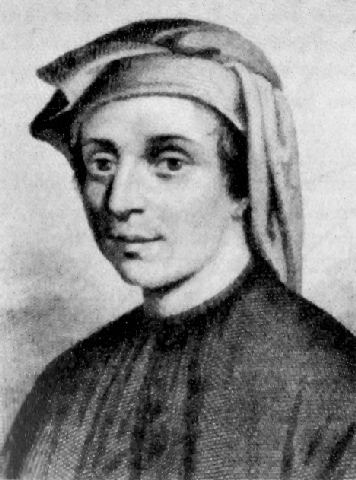
\includegraphics[width=0.5\textwidth]{Fibonacci.jpg}
    \caption{Leonardo da Pisa (1170-1240), auch Fibonacci genannt}
    \label{fig:Fibonacci}
\end{figure}

\clearpage

\begin{aufgabe}{aufgabe:0306}
Implementieren Sie eine Python-Funktion \pythoninline{def fibonacci(n)}, welche für gegebenes $n\in\N$ das $n$-te Glied der Fibonacci-Folge rekursiv berechnet. Geben Sie schliesslich die ersten $25$ Glieder der Fibonacci-Folge aus.
\end{aufgabe}

\begin{aufgabe}{aufgabe:0307}
Versuchen wir $F_{40}$ mit der Python-Funktion aus \cref{aufgabe:0306} zu berechnen, stellen wir fest, dass die Berechnung bereits recht lange dauert. Erklären Sie, warum die Berechnung der Glieder der Fibonacci-Folge mit Hilfe der \cref{definition:fibonacci} sehr aufwendig ist. Wie viele Funktionsaufrufe werden für die Berechnung von $F(5)$ benötigt? Wie viele für $F(10)$?
\end{aufgabe}

\begin{aufgabe}{aufgabe:0358}
Überlegen Sie sich, wie Sie die ersten $30$ Glieder der Fibonacci-Folge \enquote{von Hand} berechnen würden. Verwenden Sie diese Intuition um eine Python-Funktion \pythoninline{def fibonacci_fast(n)} zu schreiben, welche für gegebenes $n\in\N$ das $n$-te Glied der Fibonacci-Folge deutlich schneller und auf nicht rekursive Weise berechnet. Berechnen Sie mit Hilfe dieser Funktion das Folgeglied $F_{100}$.
\end{aufgabe}

\begin{aufgabe}{aufgabe:0309}
(*) Wir bezeichnen für $n\in\N$ mit $F_n$ die $n$-te Fibonacci-Zahl. Betrachten Sie die Gleichung
\begin{align}\label{eq:sumfib}
    F_{n+2} = 1 + \sum_{k=0}^{n} F_k
\end{align}
für $n\in\N$.
\begin{aenum}
    \item Beschreiben Sie die Aussage von \cref{eq:sumfib} in Ihren eigenen Worten.
    \item Beweisen Sie \cref{eq:sumfib}.
\end{aenum}
\end{aufgabe}

\clearpage
\section{Technische Umsetzung rekursiver Programme}\label{technisch}
In diesem Abschnitt werden wir den Übergang von der rein mathematischen Betrachtung rekursiver Algorithmen zu deren technischer Umsetzung vollziehen. Dazu betrachten wir ein Beispiel eines eleganten rekursiven Algorithmus, welcher für eine gegebene natürliche Zahl $n$ sämtliche binären Strings der Länge $n$ ausgibt. Insbesondere sollte der Algorithmus für die gegebenen Eingaben in den folgenden Testfällen die angegebenen Ausgaben erzeugen:
\begin{lstlisting}[language=Python,caption=binäre Strings rekursiv ausgeben,numbers=none]
TESTFALL 0
Eingabe: n = 0
Ausgaben:

(Es wird eine leere Zeile (leerer String) ausgegeben.)
TESTFALL 1
Eingabe: n = 1
Ausgaben:
0
1
TESTFALL 2
Eingabe: n = 2
Ausgaben:
00
01
10
11
TESTFALL 3
Eingabe: n = 3
Ausgaben:
000
001
010
011
100
101
110
111
\end{lstlisting}
Sie sind gerne eingeladen, an dieser Stelle vorerst nicht weiterzulesen und den Algorithmus selbst zu schreiben.

Unser Vorschlag für einen entsprechenden rekursiven Algorithmus ist in \cref{listing:binary} gegeben.
\begin{lstlisting}[language=Python,caption=binaryStrings,label=listing:binary]
def binaryStrings(n, w = ''):
    if n == 0:
        print(w)
        return
    binaryStrings(n-1, w + '0')
    binaryStrings(n-1, w + '1')
    #return # optional
\end{lstlisting}
Zur Vereinfachung und Konkretisierung der Beschreibung der technischen Realisation rekursiver Algorithmen werden wir sämtliche Betrachtungen dieses Abschnitts auf den Algorithmus in \cref{listing:binary} beziehen. Der Algorithmus beginnt mit dem leeren String und baut alle gesuchten Strings durch systematisches \enquote{Anhängen} von Nullen und Einsen auf. Zur Abkürzung schreiben wir anstelle von \verb|binaryString(...)| im Folgenden \verb|f(...)|.

\noindent
Betrachten wir den Aufruf \verb|f(2,'')|, um alle Strings der Länge $2$ auszugeben. Die Arbeitsschritte, welche der Funktionsaufruf \verb|f(2,'')| einleitet, sind in \cref{fig:binary} dargestellt. Die \textcolor{Green!55}{grünen} Knoten stellen Funktionsaufrufe (Aufrufe von \verb|f|) dar. Die \textcolor{Gold!85}{goldenen} Knoten stellen Aufrufe der Python-Funktion \verb|print| dar. Beim Schritt mit Nummer $\textcolor{Blue}{0}$ erfolgt der anfängliche Aufruf \verb|f(2,'')|. In diesem Aufruf wird in Programmzeile $5$ der Funktionsaufruf \verb|f(1,'0')| ausgelöst (Schritt $\textcolor{Blue}{1}$). Beachten Sie, dass der ursprüngliche Aufruf \verb|f(2,'')| seine Arbeit noch nicht abgeschlossen hat! In Programmzeile $5$ des Funktionsaufrufs \verb|f(1,'0')| wird nun der Aufruf \verb|f(0,'00')| ausgelöst. In diesem Aufruf ist die \verb|if|-Bedingung auf Programmzeile $2$ erfüllt, sodass die Ausgabe \verb|print('00')| erfolgt (Schritt $3$) und der \verb|return|-Aufruf auf Programmzeile $4$ erfolgt. Der Aufruf \verb|f(0,'00')| ist beendet und er springt zurück zum Aufruf \verb|f(1,'0')| (Schritt $\textcolor{Red}{4}$). Der Funktionsaufruf \verb|f(1,'0')| kann nun (endlich) zu Programmzeile $6$ gelangen und den Aufruf \verb|f(0,'01')| auslösen (Schritt $\textcolor{Blue}{5}$).

\begin{figure}[H]
\centering
\begin{tikzpicture}[scale=0.7, every node/.style={scale=0.7}, 
    ->, >=stealth', shorten >=1pt, auto, node distance=2.5cm, semithick]
    \tikzstyle{every state}=[fill=Green!10,draw=black,text=black]
    
    \node[state] (f2-leer) {\verb|f(2,'')|};
    \node[state] (f1-0) [below left=1.5cm and 3.4cm of f2-leer] {\verb|f(1,'0')|};
    \node[state] (f0-00) [below left=1.5cm and 1cm of f1-0] {\verb|f(0,'00')|};
    \node[state,fill=Gold!15] (p-00) [below=1.5cm of f0-00] {\verb|print('00')|};
    \node[state] (f0-01) [below right=1.5cm and 1cm of f1-0] {\verb|f(0,'01')|};
    \node[state,fill=Gold!15] (p-01) [below=1.5cm of f0-01] {\verb|print('01')|};
    \node[state] (f1-1) [below right=1.5cm and 3.4cm of f2-leer] {\verb|f(1,'1')|};
    \node[state] (f0-10) [below left=1.5cm and 1cm of f1-1] {\verb|f(0,'10')|};
    \node[state,fill=Gold!15] (p-10) [below=1.5cm of f0-10] {\verb|print('10')|};
    \node[state] (f0-11) [below right=1.5cm and 1cm of f1-1] {\verb|f(0,'11')|};
    \node[state,fill=Gold!15] (p-11) [below=1.5cm of f0-11] {\verb|print('11')|};

    \node[above=0.2cm of f2-leer] {\textcolor{Blue}{$0$ (anfänglicher Aufruf)}};

    \path   (f2-leer) edge [bend left, sloped, midway, above, Blue] node {$1$} (f1-0)
            (f1-0) edge [bend left, sloped, midway, above, Blue] node {$2$} (f0-00)
            (f0-00) edge [left, dashed] node {$3$} (p-00)
            (f0-00) edge [bend left, sloped, midway, above, Red] node {$4$} (f1-0)
            (f1-0) edge [bend left, sloped, midway, above, Blue] node {$5$} (f0-01)
            (f0-01) edge [left, dashed] node {$6$} (p-01)
            (f0-01) edge [bend left, sloped, midway, above, Red] node {$7$} (f1-0)
            (f1-0) edge [bend left, sloped, midway, above, Red] node {$8$} (f2-leer)

            (f2-leer) edge [bend left, sloped, midway, above, Blue] node {$9$} (f1-1)
            (f1-1) edge [bend left, sloped, midway, above, Blue] node {$10$} (f0-10)
            (f0-10) edge [left, dashed] node {$11$} (p-10)
            (f0-10) edge [bend left, sloped, midway, above, Red] node {$12$} (f1-1)
            (f1-1) edge [bend left, sloped, midway, above, Blue] node {$13$} (f0-11)
            (f0-11) edge [left, dashed] node {$14$} (p-11)
            (f0-11) edge [bend left, sloped, midway, above, Red] node {$15$} (f1-1)
            (f1-1) edge [bend left, sloped, midway, above, Red] node {$16$} (f2-leer)
    ;   
\end{tikzpicture}
\caption{schematische Darstellung der Arbeitsschritte zur rekursiven Ausgabe aller binären Strings der Länge $2$}
\label{fig:binary}
\end{figure}
\noindent
Erst nachdem auch \verb|f(0,'01')| seine Arbeit beendet hat (Schritte $6$ und $\textcolor{Red}{7}$), erreicht der Aufruf \verb|f(1,'0')| seine Programmzeile $7$ und springt zurück zum ursprünglichen Aufruf \verb|f(2,'')| (Schritt $\textcolor{Red}{7}$). Dieser erreicht nun Programmzeile $6$ und ruft \verb|f(1,'1')| auf (Schritt $\textcolor{Blue}{9}$). Die Schritte in dieser \enquote{rechten} Hälfte von \cref{fig:binary} lassen sich nun analog beschreiben. Erst nach der Rückgabe des Aufrufs \verb|f(1,'1')| in Schritt $\textcolor{Red}{16}$ kann schliesslich der ursprüngliche Aufruf \verb|f(2,'')| seine Arbeit beenden.

\clearpage
\begin{myBox}[Wie werden rekursive Programme in Computern realisiert?]{-}
In Computern wird für jeden Funktionsaufruf (Prozedur) ein Abschnitt im Speicher angelegt. Dieser Speicherabschnitt wird \textit{Stack-Frame} genannt. Darin darf die Funktion Speicherplatz zum Beispiel für lokale Variablen belegen. Deshalb benötigen rekursive Programme mit zahlreichen rekursiven Aufrufen viel Platz im Speicher.

Ruft eine Prozedur \verb|A| eine andere Prozedur \verb|B| auf, so wird im Stack-Frame von Prozedur \verb|B| eine sogenannte \textit{Rücksprung-Adresse} gespeichert. Diese Adresse gibt an, wo im Speicher die Prozedur \verb|A| beginnt. Dadurch wird ermöglicht, dass Prozedur \verb|B| zu Prozedur \verb|A| \enquote{zurückspringen} kann (\textit{jump and link}). Mehr Details bezüglich der Funktionsweise von Computern und rekursiven Programmen finden Sie in den hervorragenden Texten \cite{Malvino} und \cite{Sauter}.
\end{myBox}





\begin{antwort}{aufgabe:0301}
Wir beobachten, dass $13! = 13\cdot 12!$ gilt. Somit müssen wir $12!$ lediglich mit $13$ multiplizieren um $13!$ zu erhalten. Für $n\in\Nunit$ gilt allgemein
\begin{align*}
    n! = n\cdot (n-1)!.
\end{align*}
\end{antwort}


\begin{antwort}{aufgabe:0350}
Angenommen es gäbe zwei Stars $S_1$ und $S_2$ in dem Raum. Da $S_2$ ein Star ist, wird $S_2$ von allen anderen gekannt. Insbesondere kennt $S_1$ die Person $S_2$. Damit kann aber $S_1$ selbst kein Star sein. Dies ist ein Widerspruch zu unserer Annahme, dass sowohl $S_1$ als auch $S_2$ Stars sind.
\end{antwort}


\begin{antwort}{aufgabe:0351}
\begin{itemize}
    \item Frage eine beliebige Person $A$ im Raum, ob sie eine andere beliebige Person $B$ kennt.
    \item Falls $A$ die Person $B$ kennt $\Rightarrow A$ ist kein Star.
    \item Falls $A$ die Person $B$ nicht kennt $\Rightarrow B$ ist kein Star.
\end{itemize}
In jedem der Fälle haben wir mit einer einzigen Frage eine Person identifiziert, welche sicherlich kein Star ist.
\end{antwort}


\begin{antwort}{aufgabe:0352}
Der Induktionsanfang ist klar, denn für $n = 2$ benötigen wir genau zwei Fragen. Sei nun die Behauptung für ein $n\in\N$ mit $n\geq 2$ wahr. Dann gilt
\begin{align*}
    F(n+1) = F(n) + 3 = 3n-4 + 3 = 3n - 1,
\end{align*}
doch dies ist genau die Behauptung, denn $3(n+1)-4 = 3n+3-4=3n-1$.

Gemäss der soeben bewiesenen Formel sind mit unserem Vorgehen genau $F(1000) = 3\cdot 1000 - 4 = 2996$ Fragen notwendig. Beachten Sie, dass wir in keinster Weise behaupten, dass dieses Vorgehen optimal ist.
\end{antwort}


\begin{antwort}{aufgabe:0303}
\begin{lstlisting}[language=Python,caption=rekursive Potenz-Funktion]
def potenz(a,n):
    if n == 0:
        return 1
    else:
        return a * potenz(a,n-1)
\end{lstlisting}
\end{antwort}


\begin{antwort}{aufgabe:0302}
\begin{lstlisting}[language=Python,caption=rekursive Potenz-Funktion]
def factorial_loop(n):
    factorial = 1
    if n == 0:
        return factorial
    else:
        for k in range(1,n+1):
            factorial *= k
        return factorial
\end{lstlisting}
\end{antwort}


\begin{antwort}{aufgabe:0304}
\begin{aenum}
    \item Die Python-Funktion ist rekursiv definiert, da sie sich selbst aufruft.
    \item Die unbekannte Funktion multipliziert die Zahlen $m$ und $n$, realisiert also die Operation $m\cdot n$. In der Tat sieht man, dass die Funktion so lange $n$ addiert, bis $m = 0$ ist. Ein treffender Name für die Funktion wäre zum Beispiel \pythoninline{mult(m,n)}.
    \item Der Rückgabewert ist $100\cdot 50 = 5000$.
\end{aenum}
\end{antwort}


\begin{antwort}{aufgabe:0305}
\begin{lstlisting}[language=Python]
def sum_rek(L):
    if len(L) == 1:
        return L[0]
    else:
        return sum_rek(L[:-1]) + L[-1]
\end{lstlisting}
\end{antwort}


\begin{antwort}{aufgabe:0377}
\begin{lstlisting}[language=Python]
def check_palindrom(w):
    w = w.upper()
    if len(wort) <= 1:
        return True
    elif w[0] != w[-1]:
        return False
    return check_palindrom(w[1:-1])
\end{lstlisting}
oder noch kürzer:
\begin{lstlisting}[language=Python]
def check_palindrom(w):
    return (True if len(w) <= 1 else (check_palindrom(w[1:-1]) if w[0].lower() == w[-1].lower() else False))
\end{lstlisting}
\end{antwort}


\begin{antwort}{aufgabe:0308}
\begin{lstlisting}[language=Python,caption=rekursive Berechnung einer Summe]
def summe(n):
    if n == 0:
        return 0
    else:
        return n + summe(n-1)
\end{lstlisting}
\end{antwort}


\begin{antwort}{aufgabe:0311}
\begin{lstlisting}[language=Python,caption=rekursive Berechnung eines Produkts]
def produkt(n):
    if n == 1:
        return 1
    else:
        return n**3 * produkt(n-1)
\end{lstlisting}
\end{antwort}


\begin{antwort}{aufgabe:0306}
\begin{lstlisting}[language=Python,caption=rekursive Berechnung der Fibonacci-Folge]
def fibonacci(n):
    if n <= 1:
        return n
    else:
        return fibonacci(n-1) + fibonacci(n-2)
\end{lstlisting}
\noindent
Die ersten $25$ Glieder der Fibonacci-Folge lauten:
\begin{lstlisting}[language=Python,caption=die ersten 25 Glieder der Fibonacci-Folge]
0
1
1
2
3
5
8
13
21
34
55
89
144
233
377
610
987
1597
2584
4181
6765
10946
17711
28657
46368
\end{lstlisting}
\end{antwort}


\begin{antwort}{aufgabe:0307}
Die rekursiv definierte Python-Funktion aus \cref{aufgabe:0306} berechnet viele Folgeglieder mehrfach und arbeitet somit sehr \enquote{verschwenderisch}. Beispielsweise werden bei der Berechnung von $F_{40}$ die Berechnungen von $F_{39}$ und $F_{38}$ aufgerufen. Doch zur Berechnung von $F_{39}$ muss nochmals $F_{38}$ berechnet werden und so weiter. In \cref{fig:fibonacciBaum} wird gezeigt, welche Funktionsaufrufe für die rekursive Berechnung von $F(5)$ benötigt werden. Beachten Sie, dass beispielsweise der Wert fib(2) dreimal berechnet wird. Es ist klar, dass die Anzahl der benötigten Funktionsaufrufe (und somit sicherlich auch die benötigten Rechenoperationen) zur Berechnung von $F(n)$ mit wachsendem $n$ stark ansteigt. Jede Fibonacci-Zahl, ausser $F(1)$ und $F(2)$, löst jeweils zwei Funktionsaufrufe aus. Damit ist es nicht schwierig, einzusehen, dass die Anzahl $A(n)$ der Funktionsaufrufe mindestens so schnell wächst wie die Fibonacci-Folge. Die genaue Anzahl ist gegeben durch
\begin{align*}
    A(n) = 2F(n+1) - 1.
\end{align*}
In \cref{ch:Kapitel04} werden Sie sehen, dass die Fibonacci-Folge exponentiell wächst.
\begin{figure}[H]
\centering
\begin{forest}
sn edges/.style={for tree={
parent anchor=south, child anchor=north}},
sn edges
[fib(5)
[fib(4) [fib(3) [fib(2) [fib(1)] [fib(0)] ] [fib(1)] ] [fib(2) [fib(1)] [fib(0)] ]]  [fib(3) [fib(2) [fib(1)] [fib(0)] ] [fib(1)]]
]
\end{forest}
\caption{Die Anzahl Funktionsaufrufe für $F(5)$ ist 15.}
\label{fig:fibonacciBaum}
\end{figure}
\end{antwort}


\begin{antwort}{aufgabe:0358}
Die folgende Python-Funktion startet zur Berechnung von $F_n$ bei den Startwerten $F_0$ und $F_1$ und berechnet \enquote{von unten her} nacheinander (man spricht in diesem Zusammenhang von \textit{iterativer Berechnung}) die Nachfolger. Dabei werden keine Berechnungen \enquote{verschwendet}.
\begin{lstlisting}[language=Python,caption=iterative Berechnung der Fibonacci-Folge]
def fibonacci_fast(n):
    # Startwerte
    f0 = 0
    f1 = 1
    if n == 0:
        return f0
    elif n == 1:
        return f1
    
    for k in range(n-1):
        f2 = f1 + f0
        # Update
        f0 = f1
        f1 = f2
    return f2
\end{lstlisting}
Mit Hilfe dieser Funktion berechnen wir (in sehr kurzer Zeit)
\begin{align*}
    F_{100} = 354224848179261915075.
\end{align*}
\end{antwort}


\begin{antwort}{aufgabe:0309}
\begin{aenum}
    \item Die $(n+2)$-te Fibonacci-Zahl ist um $1$ grösser als die Summe der Fibonacci-Zahlen $F_0,\ldots, F_n$.
    \item Wir beweisen die Behauptung durch vollständige Induktion. Für $n = 0$ haben wir
    \begin{align*}
        1 + \sum_{k=0}^{0} F_k = 1 + F_0 = 1 + 0 = 1 = F_2.
    \end{align*}
    Wir gehen nun von der Induktionsvoraussetzung
    \begin{align*}
        F_{n+1} = 1 + \sum_{k=0}^{n-1} F_k
    \end{align*}
        aus und finden
        \begin{align*}
            &F_{n+2} = \\
            &F_n + F_{n+1} = \\
            &F_n + \lr{1 + \sum_{k=0}^{n-1}F_k} = \\
            &1 + \sum_{k=0}^{n} F_k.
        \end{align*}
\end{aenum}
\end{antwort}



\clearpage
\shipoutAnswer